\documentclass{llncs}
\usepackage[show]{ed}
\usepackage{cleveref}
\usepackage{wrapfig}
\usepackage{xspace}
\usepackage{graphicx}
\usepackage{stex-logo}
\usepackage{listings}
\definecolor{codegray}{rgb}{0.9,0.9,0.9}
\lstset{basicstyle=\sf,columns=fullflexible,backgroundcolor = \color{codegray}}

\usepackage[style=alphabetic,hyperref=auto,defernumbers=true,backend=bibtex,firstinits=true,maxbibnames=9,maxcitenames=3,isbn=false]{biblatex}
\addbibresource{kwarcpubs.bib}
\addbibresource{extpubs.bib}
\addbibresource{kwarccrossrefs.bib}
\addbibresource{extcrossrefs.bib}

% I do not want to annotate just yet.

\newcommand\ALeA{\textsf{ALeA}\xspace}
\newcommand\srf{\textsf{srify}\xspace}
\def\llangle{\langle\kern-.2em\langle}
\def\rrangle{\rangle\kern-.2em\rangle}

\title{Bulk Semantic Annotation with an Partially Known Knowledge Base}
\author{Michael Kohlhase, Jan Frederik Schaefer}
\institute{Computer Science, FAU Erlangen N\"urnberg, Germany}
\begin{document}
\maketitle
\begin{abstract}
tbw
\end{abstract}

\section{Introduction}
Arguably, dealing with large document collections is one of the key factors in the
knowledge-driven society and economy. There are currently two main contenders for machine
support in this area. Symbolic/logic-based technologies and sub-symbolic,
machine-learning-based AI, e.g. via LLMs or chatbots; they have complementary strengths
and challenges: Symbolic technologies offer precision and explainability out of the box,
but face scalability challenges, because the prerequisite background knowledge has to be
(manually) formalized. ML-based approaches can be trained on all data of the Internet, but
face challenges in precision and explanations. Aarne Ranta matches these profiles to the
notion of \textbf{producer tasks} -- i.e. tasks where precision is key, but limited
coverage ($10^{3\pm1}$ concepts) is OK; e.g. for multi-language/variant manuals for very
expensive tool machines -- and \textbf{consumer tasks}, where coverage is key and
precision secondary; e.g. for consumer-grade machine translation like \textsf{Google
  translate} in \cite{Ranta:atcp17}.

In this paper, we address tools that help attack the coverage problem in symbolic/semantic
approaches in practice. The producer task we use as a case study is that of adaptive
learning assistants for MINT subjects, concretely the \ALeA system
\cite{BerBetChu:lssmkm23}, which uses \sTeX \cite{MueKo:sdstex22,sTeX:github:on} -- a
variant of {\LaTeX} that allows to embed semantic annotations -- for a knowledge
representation and generates learner-adaptive learning objects instrumented with
learning-support interactions from that. The \textbf{\sTeX/\ALeA content commons}
\ednote{MK@MK: continue to describe the size and distribution, and
  authorship}\ednote{explain the \textbf{domain model} (the SMGloM) and the
  \textbf{formulation model} (cf. \cite{BerBetChu:lssmkm23}) in the commons and give their
  releative sizes.}

We contend that while education -- especially higher education -- as a whole is a
wide-coverage task for society education of individual learners in specific domains --
especially, if we want to tailor the educational offerings to said individual/domain -- is
a producer task, at least until ML-based methods reach the precision and explainability
required by the ethics of teaching.

\section{Semantic Authoring in a Content Common}

The main practical problem of annotating presentational {\LaTeX} course materials into
semantic documents that carry enough information to support meaningful learning support
services is to add semantic references to technical terms from the domain jargon. Take for
instance a learning object like the paragraph in \cref{fig:lo}, where we want to annotate
the the term ``state space'' with the (semantic) concept of a ``state space of a search
problem''. The latter can either be defined earlier in the course or in the domain mode
(or both).

\begin{figure}[ht]\centering
  \fbox{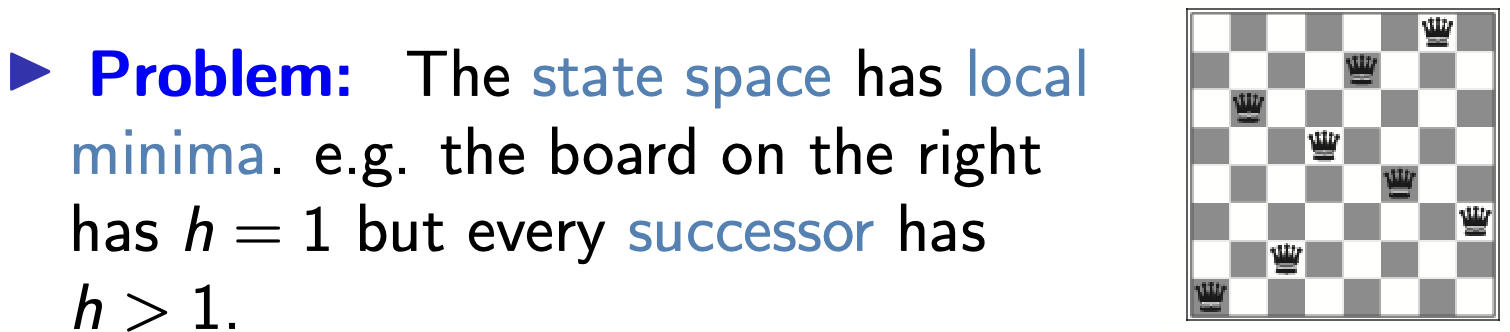
\includegraphics[width=8cm]{../img/problem}}
  \caption{An annotated Learning Object from an AI Lecture}\label{fig:lo}
\end{figure}

Concretely this is about converting the {\LaTeX} string\ednote{add numbers, start with 3
  so that corresponding lines with the next listing.}
\begin{lstlisting}[language={[LaTeX]TeX}]
\item \blue{Problem:} The state space has local minima, e.g. the board on the
  right has $h=1$ but every successor has $h>1$. 
\end{lstlisting}
into the (partially annotated item:
\begin{lstlisting}[language={[LaTeX]TeX},morekeywords={sn,importmodule}]
\importmodule[smglom/search]{mod?state-space}
[...]  
\item \blue{Problem:} The \sn{state space} has local minima, e.g. the
  board on the right has $h=1$ but every successor has $h>1$. 
\end{lstlisting}
Concretely, the author has to remember the module for the term ``state space'' from
\cref{fig:state-space}, the symbol name \lstinline|state space|, annotate it with the
\sTeX macro \lstinline|\sn{...}|, and add the module import in the first line (unless it
is already imported). In this case the symbol name happens to be the same as its English
verbalization, otherwise we would have to use
\lstinline[mathescape]|\sr{$\llangle symbol name\rrangle$}{state space}|.

\begin{figure}[ht]\centering
  \fbox{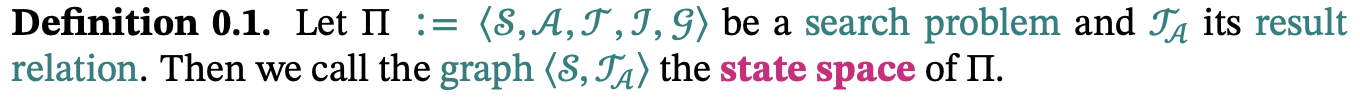
\includegraphics[width=12cm]{../img/state-space}}
  \caption{The definition of the term ``state space'' from the domain model}\label{fig:state-space}
\end{figure}

For this, the author has to be aware ``state space'' is a technical term, that the module
from \cref{fig:state-space} exists, know the symbol name and its URL, and manage
reduncancy of the imports. At ca 150.000 words in a semester's words of lecture notes and
ca. 10-15\% of technical terms a rather daunting task.

\sTeX authoring is already supported by an VSCode IDE plugin \cite{sTeX-IDE:git} that
analyzes annotations on the fly, displays the underlying reference semantics, reports
errors and redundancies, and even offers a concept search interface. But these only offer
support already annotated terms, so they do not solve the annotation problem above.

\section{The \srf System}

The \srf system (see \cite{stextools:git} is a simple command-line tool that creates a
database of symbol-verbalization pairs\ednote{explain that first}, analyzes \sTeX source
files and then steps through all word occurrences in the document that share the stem with
a verbalization in the database. For each such word, the user is presented with an
annotation choice and interactions that allow to fine-tune the wordwise annotation
workflow.

As \srf addresses mostly power-users, the UI of \srf is command-line based, much like the
early \textsf{ispell} system, see\ednote{continue}

\section{Practical Evaluation}

In our experience, the step-through workflow for annotating term references for symbols
from the domain model is almost an order of magnitude more efficient than writing the
annotations and imports by hand, even for annotators who are familiar with the domain
model. For annotators unfamiliar with the domain model, the unassisted annotation task is
almost infeasible, and the average unfamiliarity naturally grows with the domain
model. The symbol disambiguation process -- on average a word induces $n$\ednote{MK@FS: we
  should try to measure this: for every verbalization (i.e. symbol/word pair) we should
  compute the ratio of those words with the same stem.} choices is still manageable,
requires considerable concentration and domain knowledge, but little knowledge of the
domain model flexiformalization.

The command-line interface is simple and responsive and gives all the necessary
information in a single glance if underlying shell area exceeds ca. $80\times 35$
characters. It is very much geared towards annotating existing documents with respect to a
relatively complete -- pre-existing -- domain model, and it seems unlikely that a more
sophisticated UI would add value for this use-case.

For less complete domain models we have to skip too many terms that should ultimately be
annotated and annotation efficiency suffers. This is currently the case for all
non-English languages in the \sTeX corpus we work with. Coverage in German is only about
half of that of English and we can already see the practical effects. We have also
experimented with a Slovene introductory math book, and it seems clear that apart from
having to introduce a Slovene stemmer\ednote{MK@FS: there is one for python at
  \url{https://repo.ijs.si/pboskoski/slo_stemmer}}, we would need to manually annotate all
definienda in the book before we can harvest the symbol/verbalization pairs which are a
prerequisite for annotation.

The current interface is not well-suited for on-the-fly annotation while editing while
authoring. For that, the underlying information (the symbol/verbalization pairs harvested
from the domain model) can be integrated into any IDE. In fact we plan to do this for the
next version of the sTeX plugin for VSCode \cite{sTeX-IDE:git}.


\section{Conclusion}

In this system description we have presented the \srf tool, a command-line tool
\ednote{continue}

In an earlier attempt to support semantic annotation in IDEs, we tried named-entity
recognition (NER) for classification of ``likely annotation candidate words''
\cite{hutterer:msc23}, however this classification was not precise enough in the
distinction in ``technical terms'' and ordinary english noun phrases and named entities --
the relevant task for annotation, and so made it impractical, especially, since it could
not enter the actual annotations and import directives automatically. But maybe using the
NER-based approach, after the \srf annotation process might change the tradeoffs
involved. In any case, the overall workflow suggested by the NER-based approach --
especially after the verbalizations covered by the existing domain model\ednote{introduce
  in the definition above that the domain model is all definitions, not only in the
  smglom?} -- is geared towards adding modules and symbols -- the ones discovered by NER
-- to the domain model. 



\printbibliography
\end{document}

%%% Local Variables:
%%% mode: latex
%%% TeX-master: t
%%% End:

% LocalWords:  tbw Aarne Ranta
